\documentclass[a4paper]{article}
\usepackage[utf8]{inputenc}
\usepackage{geometry}
\usepackage{amsmath}
\pdfpagewidth
\paperwidth
\pdfpageheight
\paperheight
\usepackage{booktabs}
\usepackage{graphicx}
\usepackage{subfig}
\usepackage{verbatim}
\newcommand*{\unit}[1]{\ensuremath{\mathrm{\,#1}}}
\usepackage{amsthm}
\usepackage{epsfig}
\usepackage{fancyhdr} 
\usepackage{amsmath,amssymb}
\usepackage{amscd} 
\usepackage[T1]{fontenc} 
\usepackage[utf8]{inputenc} 
\usepackage[usenames,dvipsnames]{xcolor}
\usepackage{graphicx,color,listings}
\usepackage{hologo}
\frenchspacing 
\usepackage{float}
\usepackage{geometry}
\usepackage{rotating}
\usepackage{caption}
\captionsetup{labelformat=empty, textfont=sl}
\usepackage{placeins}
\usepackage{hyperref}
\frenchspacing
\title{Esperienza Laboratorio di Fisica Medica: Raggi X}
\author{Simone Lossano, Lorenzo Marini, Jake Harold Pensavalle}
\begin{document}
	\maketitle
	\newpage
	\tableofcontents
	\newpage
%%%%%%%%%%%%%%%%%%%%%%%%%%%%%%%%%%%%%%

%%%%%%%%%%%%%%%%%%%%%%%%%%%%%%%%%%%%%%
\section{Riproducibilità della radiazione emessa dal tubo}


In questa prima sezione si prende manualità con lo strumento facendo una verifica della riproducibilità del fascio. Dai grafici prodotti si vede ad occhio che il fascio ha piccole variazioni e si può considerare il fascio abbastanza riproducibile, anche se dal test dell' $R^{2}$ risulta riproducibile l'acquisizione a 80 kVp.
\begin{center} 
		
		\begin{tabular}{lcccccc}
			\hline
			\hline
			\textbf{kVp}	& \textbf{coefficiente angolare}& \textbf{intercetta}& \textbf{media}& \textbf{deviazione standard}& \textbf{$R^{2}$} 	 \\
			\hline
			\hline
			40	&0.005&9.783&9.789&0.010&0.247 	\\
			60	&0.020&30.820&30.880&0.038&0.289\\
			80	&0.150&53.970&54.420&0.743&0.867 \\
			90	&0.030&67.790&67.880&0.068&0.247\\
			
			\hline
			\hline
		\end{tabular}
		\linebreak
		\emph{Tab.1: risultati fit lineare dei punti acquisiti per la riproducibilità della radiazione.} 
	\end{center}

\begin{figure}[H]%
    \centering
    \subfloat[]{{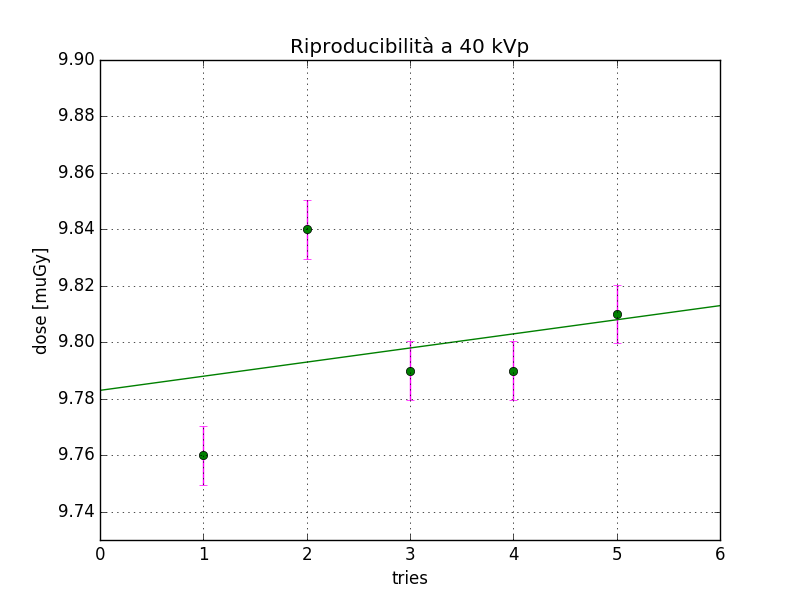
\includegraphics[width=5cm]{riproducibilita40kvp} }}%
    \qquad
    \subfloat[]{{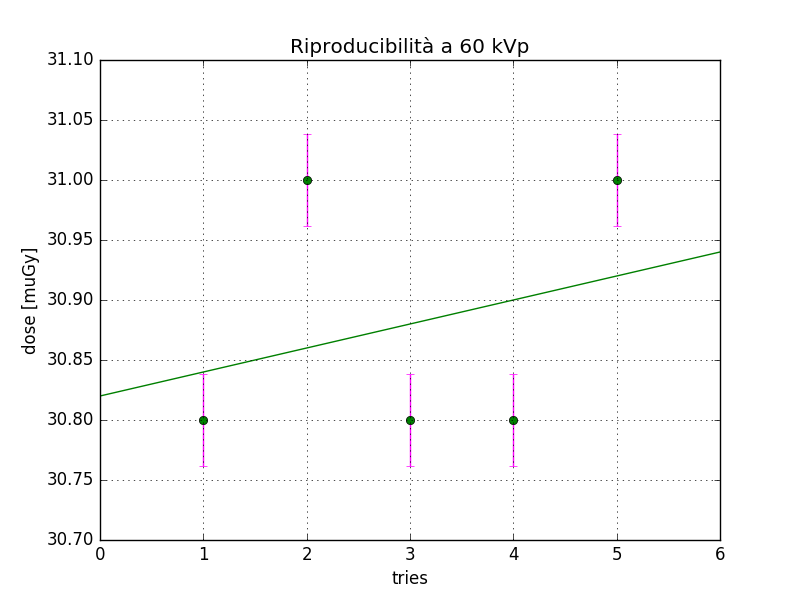
\includegraphics[width=5cm]{riproducibilita60kvp} }}%
    \qquad
    \subfloat[]{{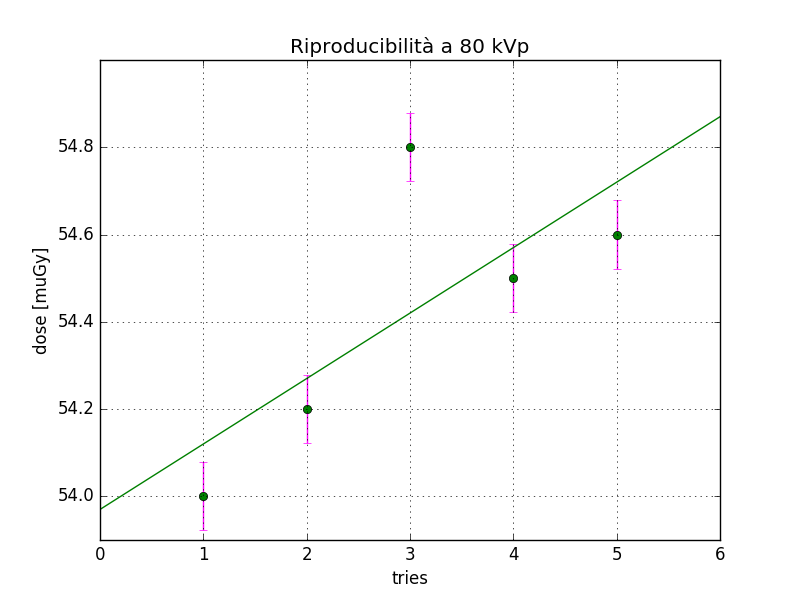
\includegraphics[width=5cm]{riproducibilita80kvp}}}%
    \qquad
    \subfloat[]{{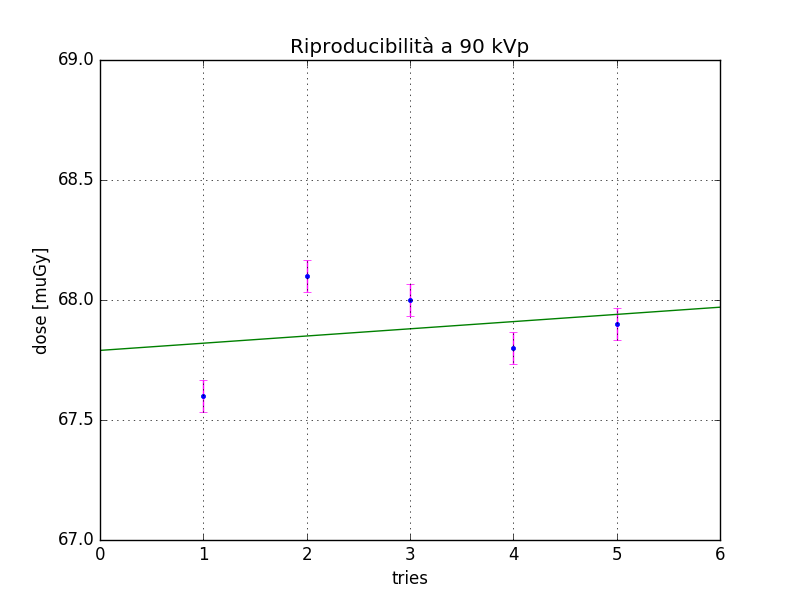
\includegraphics[width=5cm]{riproducibilita90kvp}}}%
    
   \caption{Grafici Riproducibilità della radiazione a vari valori di kVp.}%
    \label{fig:1}%
\end{figure}

\newpage
%%%%%%%%%%%%%%%%%%%%%%%%%%%%%%%%%%%%%%
\section{Andamento della dose in aria in funzione di diversi parametri}
In questa sezione si studia l'andamento della Dose in aria in funzione di vari parametri, quali \textbf{la corrente anodica}, \textbf{il tempo di esposizione}, \textbf{la differenza di potenziale tra gli elettrodi} e \textbf{distanza fuoco-camera di ionizzazione}.                           
\subsection{Linearità Dose in aria in funzione della corrente anodica}
Dall' \textbf{interpolazione} si vede che i dati sono fittati meglio da una funzione lineare, grazie al valore più prossimo a 1 di $R^{2}$. Una migliore analisi futura può essere condotta eliminando gli outlier.
\begin{figure}[H]
\centering
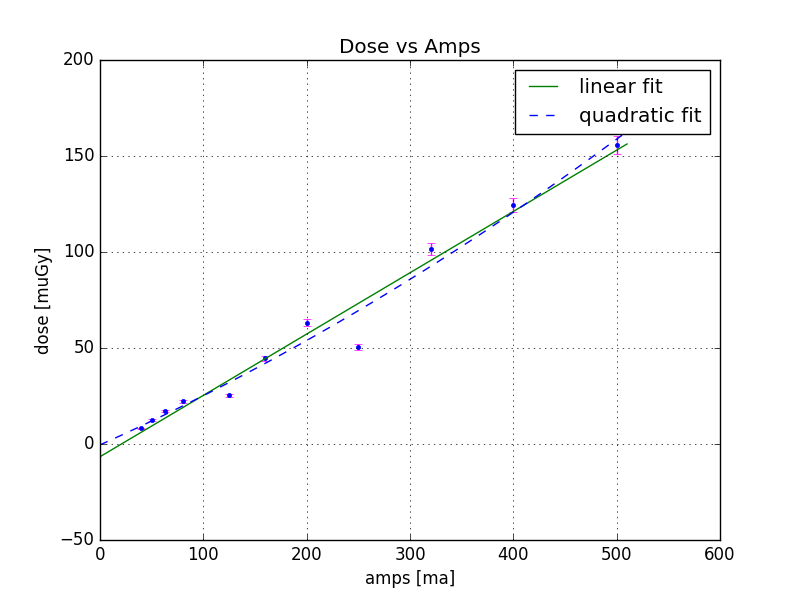
\includegraphics[width=0.75\textwidth]{dosevsamps.png}
\caption{Dose in funzione della corrente anodica.}
\end{figure}

\begin{center} 
		
		\begin{tabular}{lccccc}
			\hline
			\hline
			\textbf{Modello}	& \textbf{coefficiente di grado 2}& \textbf{coefficiente di grado 1}& \textbf{intercetta}&  \textbf{$R^{2}$} 	 \\
			\hline
			\hline
			Lineare	&-&0.319&-6.619&0.986	\\
			Quadratico	&0.0001&0.241&-0.469&0.975\\
			
			
			\hline
			\hline
		\end{tabular}
		\linebreak
		\emph{Tab.2: risultati fit lineare e quadratico dei punti acquisiti per la Dose in funzione della corrente anodica.} 
	\end{center}

%%%%%%%%%%%%%%%%%%%%%%%%%%%%%%%%%%%%%%
\subsection{Linearità Dose in aria in funzione della tempo di esposizione}
Dall' \textbf{interpolazione} si vede che i dati sono fittati meglio da una funzione lineare, grazie al valore più prossimo a 1 di $R^{2}$. Anche qui una migliore analisi futura può essere condotta eliminando gli outlier.
\begin{figure}[H]
\centering
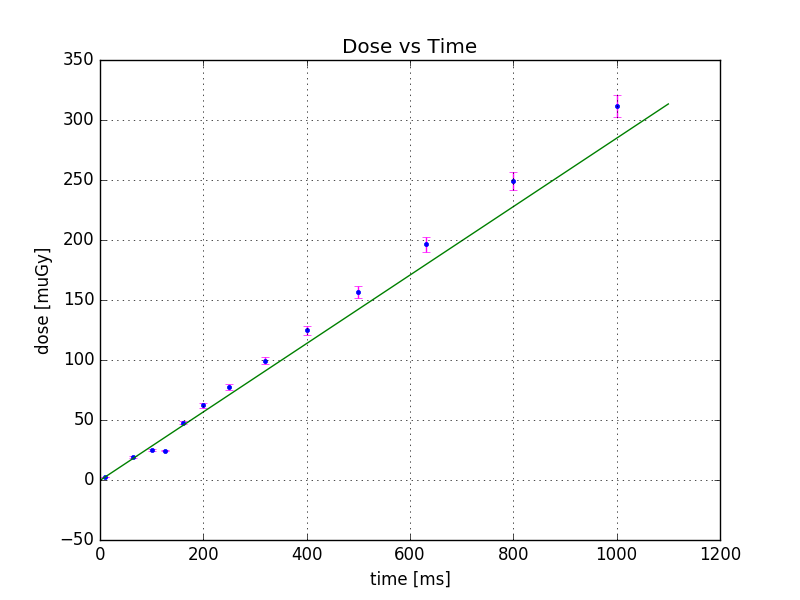
\includegraphics[width=0.75\textwidth]{dosevstime.png}
\caption{Dose in funzione del tempo di esposizione.}
\end{figure}

\begin{center} 
		
		\begin{tabular}{lccccc}
			\hline
			\hline
			\textbf{Modello}	& \textbf{coefficiente di grado 2}& \textbf{coefficiente di grado 1}& \textbf{intercetta}&  \textbf{$R^{2}$} 	 \\
			\hline
			\hline
			Lineare	&-&0.300&-3.616&0.999	\\
			Quadratico	&0.0001&0.326&-4.791&0.998\\
			
			
			\hline
			\hline
		\end{tabular}
		\linebreak
		\emph{Tab.3: risultati fit lineare e quadratico dei punti acquisiti per la Dose in funzione del tempo di esposizione.} 
	\end{center}
%%%%%%%%%%%%%%%%%%%%%%%%%%%%%%%%%%%%%%
\subsection{Linearità Dose in aria in funzione della differenza di potenziale tra gli elettrodi}
Dall' \textbf{interpolazione} si vede che i dati sono fittati meglio da una funzione \textbf{quadratica}, grazie al valore più prossimo a 1 di $R^{2}$. 

\begin{figure}[H]
\centering
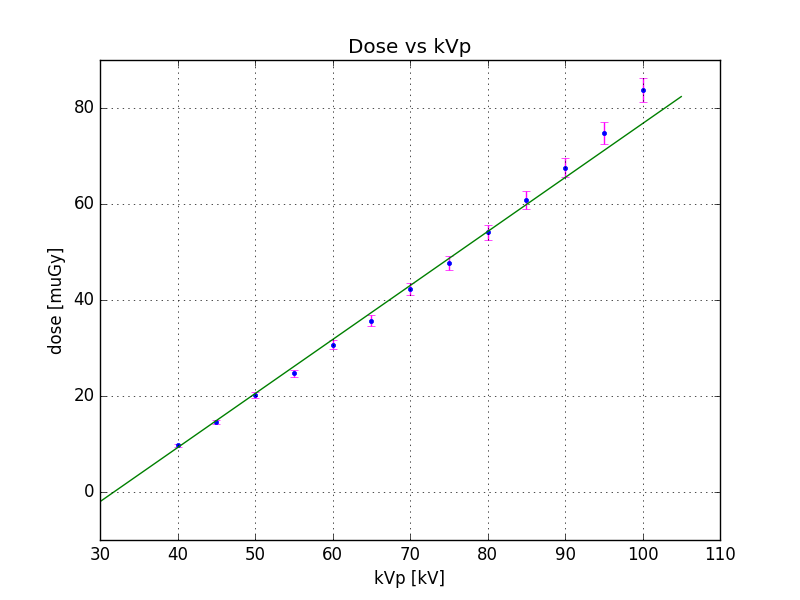
\includegraphics[width=0.75\textwidth]{dosevsvolts.png}
\caption{Dose in funzione della differenza di potenziale tra gli elettrodi.}
\end{figure}

\begin{center} 
		
		\begin{tabular}{lccccc}
			\hline
			\hline
			\textbf{Modello}	& \textbf{coefficiente di grado 2}& \textbf{coefficiente di grado 1}& \textbf{intercetta}&  \textbf{$R^{2}$} 	 \\
			\hline
			\hline
			Lineare	&-&1.211&-41.165&0.997	\\
			Quadratico	&0.005&0.470&-17.099&0.999\\
			
			
			\hline
			\hline
		\end{tabular}
		\linebreak
		\emph{Tab.4: risultati fit lineare e quadratico dei punti acquisiti per la Dose in funzione della differenza di potenziale tra gli elettrodi.} 
	\end{center} 
%%%%%%%%%%%%%%%%%%%%%%%%%%%%%%%%%%%%%%
\subsection{Linearità Dose in aria in funzione della distanza fuoco-camera a ionizzazione}
Come modello si è utilizzato \begin{equation}
Dose=A\frac{C}{r^{2}}+B
\end{equation}
Con A e B parametri stimati dal fit.
\begin{figure}[H]
\centering
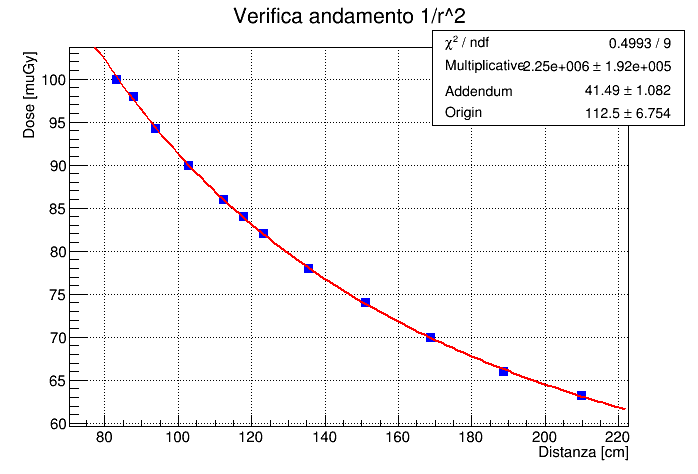
\includegraphics[width=0.75\textwidth]{Dosevsdistancewithpar.png}
\caption{Dose in funzione della distanza fuoco-camera a ionizzazione. Grazie al valore del $\chi^{2}_{redux}$ di 0.454 non si ha ragione di rigettare l'ipotesi che il modello descriva bene i dati.}
\end{figure}


\newpage

%%%%%%%%%%%%%%%%%%%%%%%%%%%%%%%%%%%%%%
\section{Calcolo degli spessori emivalenti (HVL)}
In questa sezione si stimano i valori di HVL per ricavare il coefficiente di assorbimento dell' alluminio con l'interpolazione, infatti l'andamento è esponenziale solo per valori elevati dello spessore. Dato HVL per stimare il coefficiente di assorbimento si usa: \begin{equation}
\mu =\frac{0.693}{HVL}
\end{equation} 
Si riportano il grafico, il modello e il confronto tra valori attesi e valori sperimentali a vari valori di kVp e a ampiezze del fascio diverse.  
\begin{figure}[H]
\centering
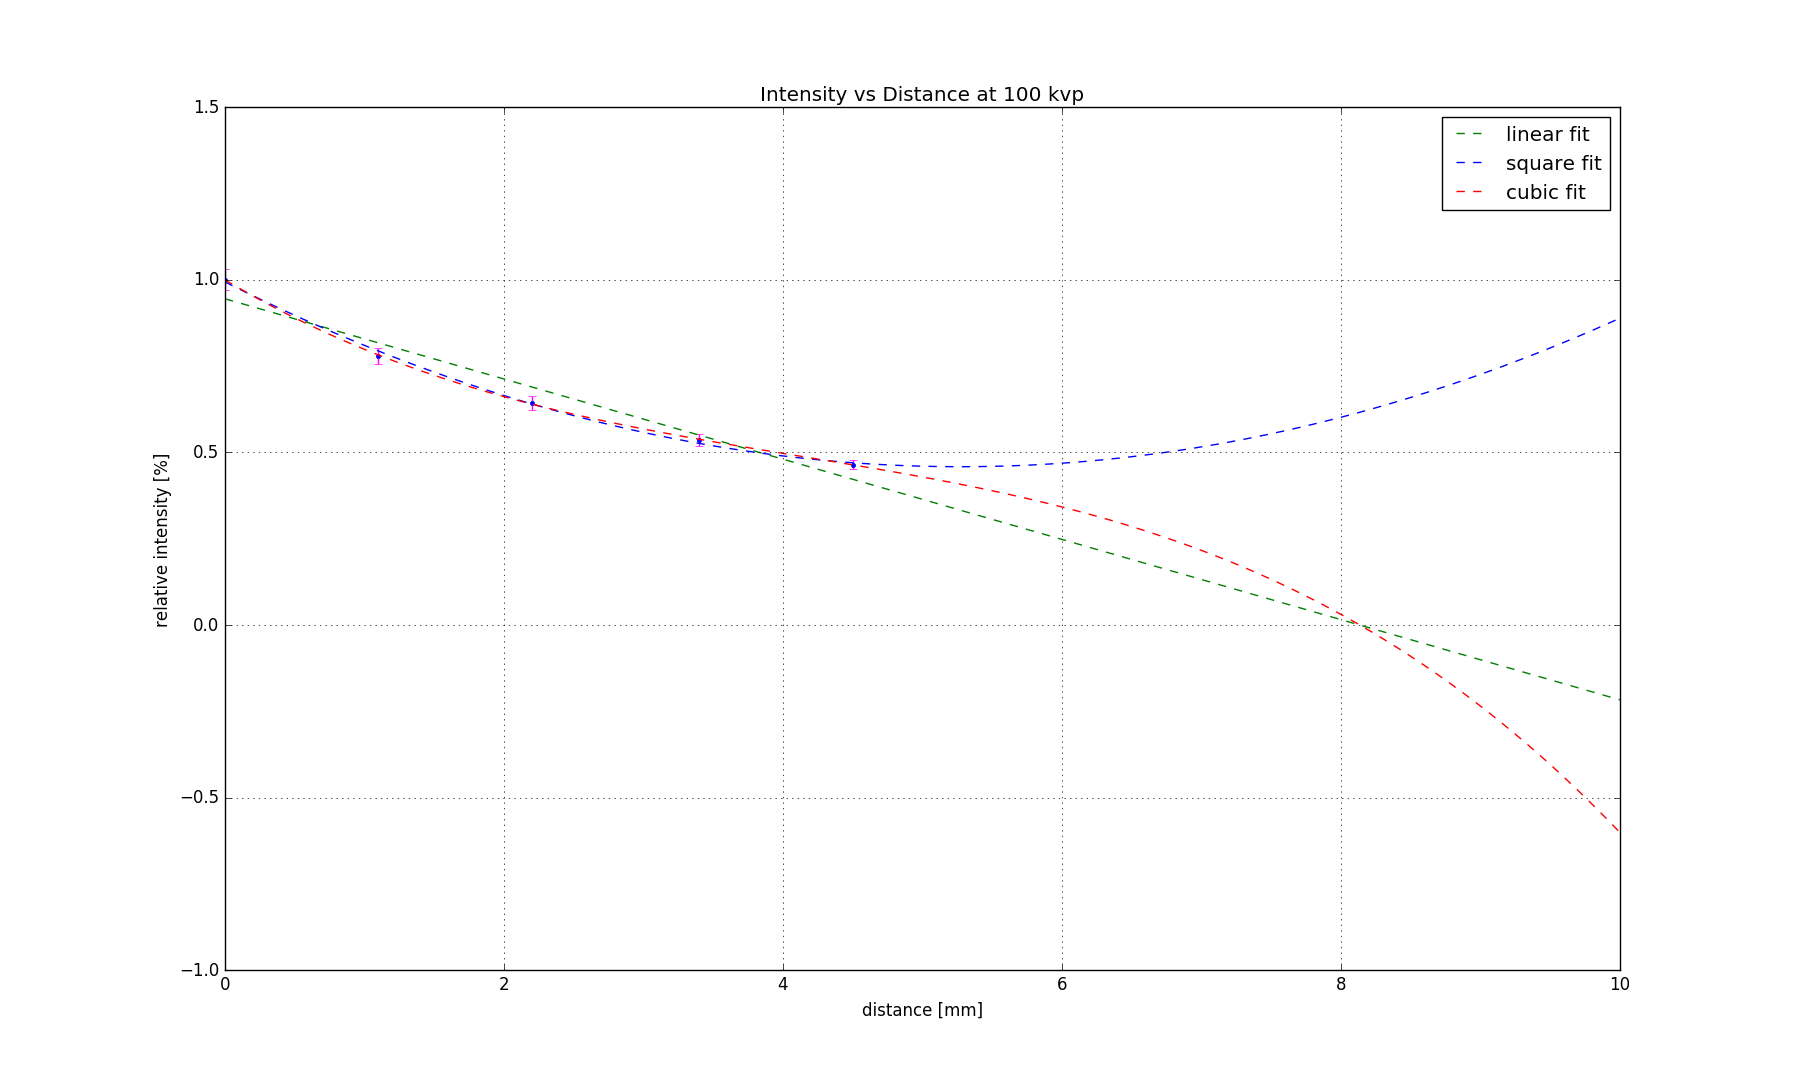
\includegraphics[width=0.75\textwidth]{hvl100pvk.png}
\caption{Intensità del fascio incidente in funzione dello spessore a 100 kVp con fascio stretto.}
\end{figure}

\begin{center} 
		
		\begin{tabular}{lccccccc}
			\hline
			\hline
			\textbf{Modello}	& \textbf{coeff. grado 4}&\textbf{coef. grado 3}&\textbf{coef. grado 2}& \textbf{coef. grado 1}& \textbf{intercetta}&  \textbf{$R^{2}$} 	 \\
			\hline
			\hline
			Lineare	&-&-&-&-0.137&0.949&0.894	\\
			Cubico	&-&0.001&0.022&-0.197&0.988&0.998\\
			Quartico &0.0001&-0.003&0.037&-0.229&0.998&0.999\\
			
			\hline
			\hline
		\end{tabular}
		\linebreak
		\emph{Tab.5: risultati fit lineare, cubico e quartico  dei punti acquisiti per la intensità di radiazione (proporzionale alla dose) in funzione dello spessore . Si vede dal valore di $R^{2}$ che il fit quartico descrive meglio i dati} 
	\end{center} 



\begin{figure}[H]
\centering
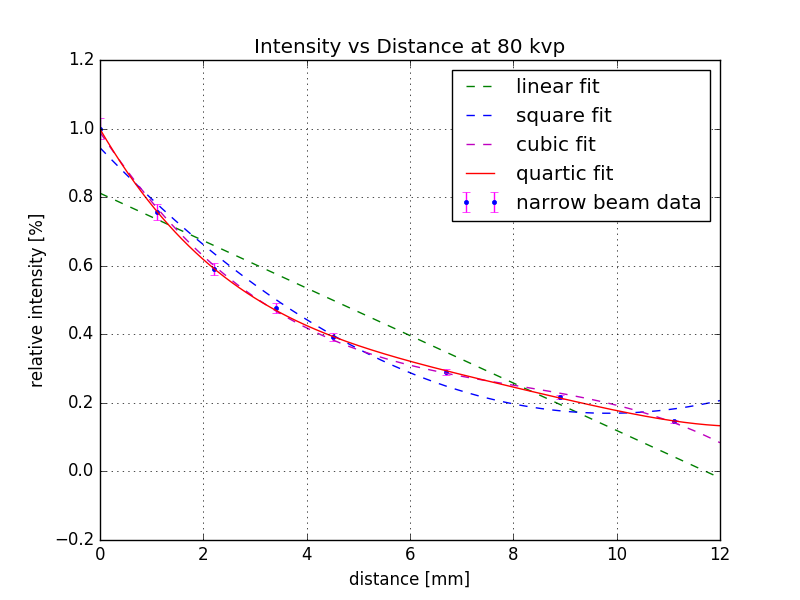
\includegraphics[width=0.75\textwidth]{hvl80pvk.png}
\caption{Intensità del fascio incidente in funzione dello spessore a 80 kVp con fascio stretto.}
\end{figure}

\begin{center} 
		
		\begin{tabular}{lccccccc}
			\hline
			\hline
			\textbf{Modello}	& \textbf{coeff. grado 4}&\textbf{coef. grado 3}&\textbf{coef. grado 2}& \textbf{coef. grado 1}& \textbf{intercetta}&  \textbf{$R^{2}$} 	 \\
			\hline
			\hline
			Lineare	&-&-&-&-0.069&0.811&0.868	\\
			Cubico	&-&-0.001&0.025&-0.227&0.989&0.998\\
			Quartico &0.0001&-0.003&0.04&-0.258&0.998&0.999\\
			
			\hline
			\hline
		\end{tabular}
		\linebreak
		\emph{Tab.6: risultati fit lineare, cubico e quartico  dei punti acquisiti per la intensità di radiazione (proporzionale alla dose) in funzione dello spessore . Si vede dal valore di $R^{2}$ che il fit quartico descrive meglio i dati} 
	\end{center} 


\begin{figure}[H]
\centering
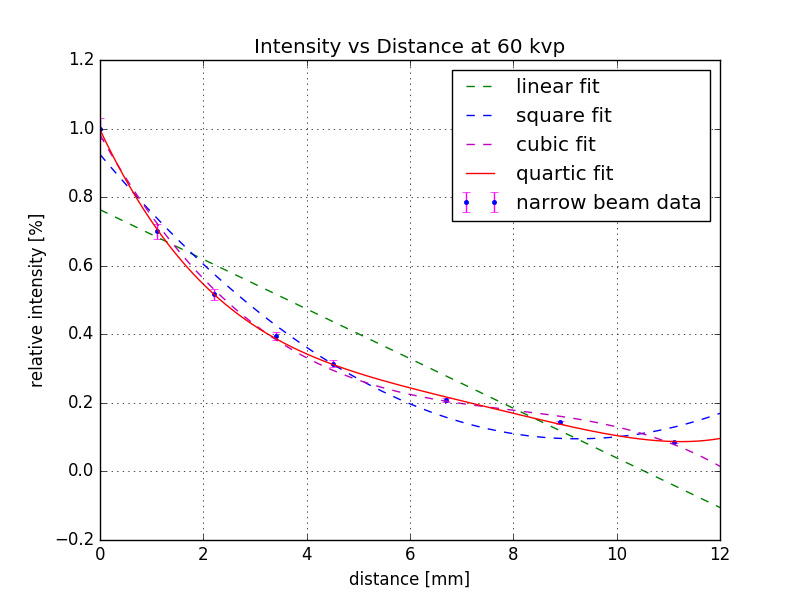
\includegraphics[width=0.75\textwidth]{hvl60pvk.png}
\caption{Intensità del fascio incidente in funzione dello spessore a 60 kVp con fascio stretto.}
\end{figure}

\begin{center} 
		
		\begin{tabular}{lccccccc}
			\hline
			\hline
			\textbf{Modello}	& \textbf{coeff. grado 4}&\textbf{coef. grado 3}&\textbf{coef. grado 2}& \textbf{coef. grado 1}& \textbf{intercetta}&  \textbf{$R^{2}$} 	 \\
			\hline
			\hline
			Lineare	&-&-&-&-0.072&0.763&0.827	\\
			Cubico	&-&-0.001&-0.031&-0.267&0.982&0.997\\
			Quartico &0.0002&-0.005&0.056&-0.319&0.997&0.999\\
			
			\hline
			\hline
		\end{tabular}
		\linebreak
		\emph{Tab.7: risultati fit lineare, cubico e quartico  dei punti acquisiti per la intensità di radiazione (proporzionale alla dose) in funzione dello spessore . Si vede dal valore di $R^{2}$ che il fit quartico descrive meglio i dati} 
	\end{center} 


\begin{figure}[H]
\centering
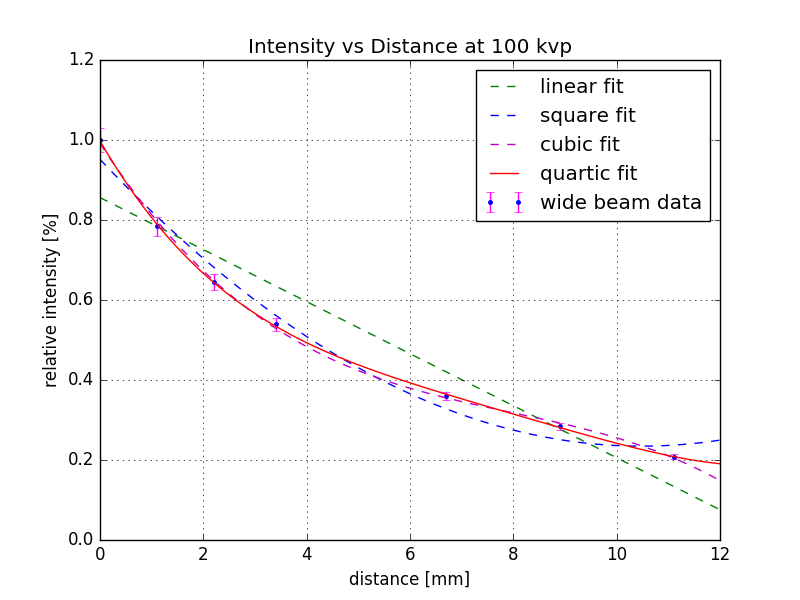
\includegraphics[width=0.75\textwidth]{hvl100pvkwide.png}
\caption{Intensità del fascio incidente in funzione dello spessore a 100 kVp con fascio aperto.}
\end{figure}

\begin{center} 
		
		\begin{tabular}{lccccccc}
			\hline
			\hline
			\textbf{Modello}	& \textbf{coeff. grado 4}&\textbf{coef. grado 3}&\textbf{coef. grado 2}& \textbf{coef. grado 1}& \textbf{intercetta}&  \textbf{$R^{2}$} 	 \\
			\hline
			\hline
			Lineare	&-&-&-&-0.065&0.856&0.991	\\
			Cubico	&-&-0.001&0.022&-0.199&0.992&0.984\\
			Quartico &0.0009&0.003&0.034&-0.223&0.998&0.999\\
			
			\hline
			\hline
		\end{tabular}
		\linebreak
		\emph{Tab.8: risultati fit lineare, cubico e quartico  dei punti acquisiti per la intensità di radiazione (proporzionale alla dose) in funzione dello spessore . Si vede dal valore di $R^{2}$ che il fit quartico descrive meglio i dati} 
	\end{center} 

\begin{figure}[H]
\centering
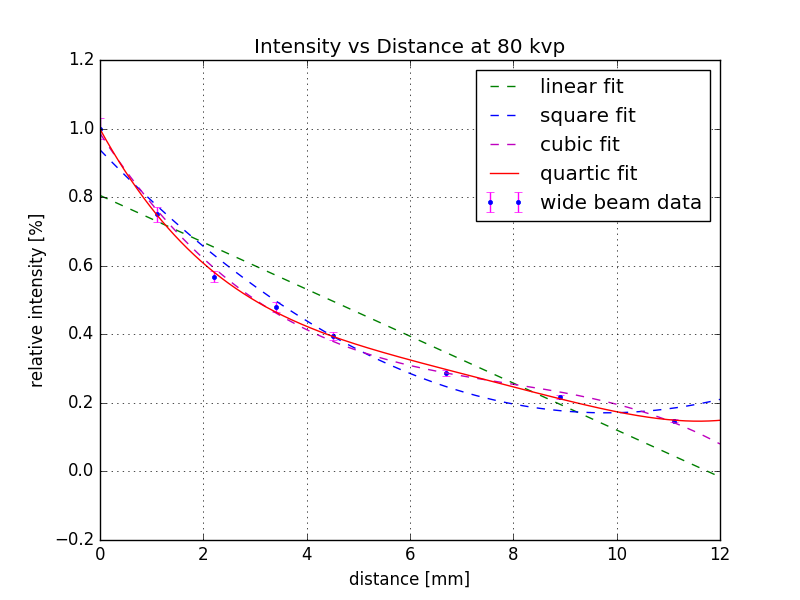
\includegraphics[width=0.75\textwidth]{hvl80kvpwide.png}
\caption{Intensità del fascio incidente in funzione dello spessore a 80 kVp con fascio aperto.}
\end{figure}

\begin{center} 
		
		\begin{tabular}{lccccccc}
			\hline
			\hline
			\textbf{Modello}	& \textbf{coeff. grado 4}&\textbf{coef. grado 3}&\textbf{coef. grado 2}& \textbf{coef. grado 1}& \textbf{intercetta}&  \textbf{$R^{2}$} 	 \\
			\hline
			\hline
			Lineare	&-&-&-&-0.157&0.938&0.862	\\
			Cubico	&-&-0.001&0.026&-0.238&0.986&0.997\\
			Quartico &0.0001&-0.004&0.047&-0.274&0.999&0.999\\
			
			\hline
			\hline
		\end{tabular}
		\linebreak
		\emph{Tab.9: risultati fit lineare, cubico e quartico  dei punti acquisiti per la intensità di radiazione (proporzionale alla dose) in funzione dello spessore . Si vede dal valore di $R^{2}$ che il fit quartico descrive meglio i dati} 
	\end{center} 




\begin{figure}[H]
\centering
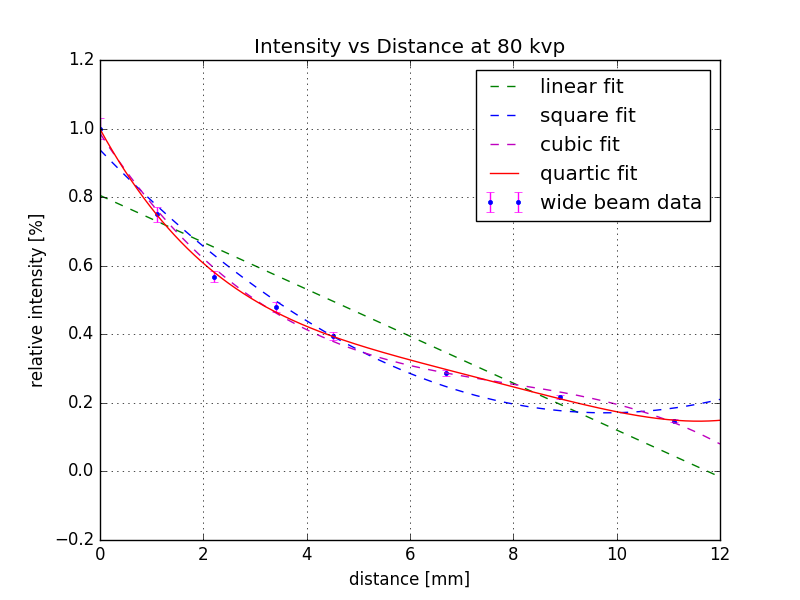
\includegraphics[width=0.75\textwidth]{hvl80kvpwide.png}
\caption{Intensità del fascio incidente in funzione dello spessore a 60 kVp con fascio aperto.}
\end{figure}

\begin{center} 
		
		\begin{tabular}{lccccccc}
			\hline
			\hline
			\textbf{Modello}	& \textbf{coeff. grado 4}&\textbf{coef. grado 3}&\textbf{coef. grado 2}& \textbf{coef. grado 1}& \textbf{intercetta}&  \textbf{$R^{2}$} 	 \\
			\hline
			\hline
			Lineare	&-&-&-&-0.072&0.762&0.824	\\
			Cubico	&-&-0.001&0.032&-0.268&0.980&0.996\\
			Quartico &0.0002&-0.005&0.057&-0.322&0.995&0.999\\
			
			\hline
			\hline
		\end{tabular}
		\linebreak
		\emph{Tab.10: risultati fit lineare, cubico e quartico  dei punti acquisiti per la intensità di radiazione (proporzionale alla dose) in funzione dello spessore . Si vede dal valore di $R^{2}$ che il fit quartico descrive meglio i dati} 
	\end{center} 
\subsection{Confronto coefficienti di assorbimento: Aspettati Vs Sperimentali }
Avendo trovato la funzione che meglio descrive i dati sperimentali si può stimare HVL di ogni acquisizione, con incertezza associata alla lettura del valore sul display di Python, e calcolare il coefficiente di assorbimento con la formula (2) e confrontarlo col valore tabulato.
\begin{center} 
		
		\begin{tabular}{lccccc}
			\hline
			\hline
			\textbf{Apertura Fascio} &\textbf{kVp}	& \textbf{HVL [cm]}&\textbf{$\frac{\mu}{\rho}_{exp}[\frac{cm^{2}}{gr}]$}&\textbf{$\frac{\mu}{\rho}_{Theo}[\frac{cm^{2}}{gr}]$} 	 \\
			\hline
			\hline
			Stretto	& 100 &	$0.388 \pm 0.001$ &$0.622 \pm 0.001$&0.569 \\
			Stretto	& 80 &	$0.305 \pm 0.001$ &$0.841 \pm 0.001$&0.569 \\
			Stretto	& 60 &	$0.233 \pm 0.001$ &$1.101 \pm 0.001$&1.128 \\
			Largo	& 100 &	$0.394 \pm 0.001$ &$0.659 \pm 0.001$&0.569 \\
			Largo	& 80 &	$0.298 \pm 0.001$ &$0.861 \pm 0.001$&0.569 \\
			Largo	& 60 &	$0.231 \pm 0.001$ &$1.111 \pm 0.001$&1.128 \\
			
			
			\hline
			\hline
		\end{tabular}
		\linebreak
		\emph{Tab.11: Confronto tra assorbimento massico sperimentale e tabulato. Le discrepanze sono dovute al fatto che il coefficiente d'assorbimento trovato è un coefficiente d'assorbimento medio. Inoltre per gli 80 kVp si riporta il valore più vicino tabulato, ma i valori tabulati non sono riportati a tutte le energie.} 
\end{center}
\section{Effetto Heel}
Facendo variare la posizione della camera a gas abbiamo verificato che l'energia del fascio non è la stessa in prossimità del catodo e dell'anodo.
\begin{figure}[H]
\centering
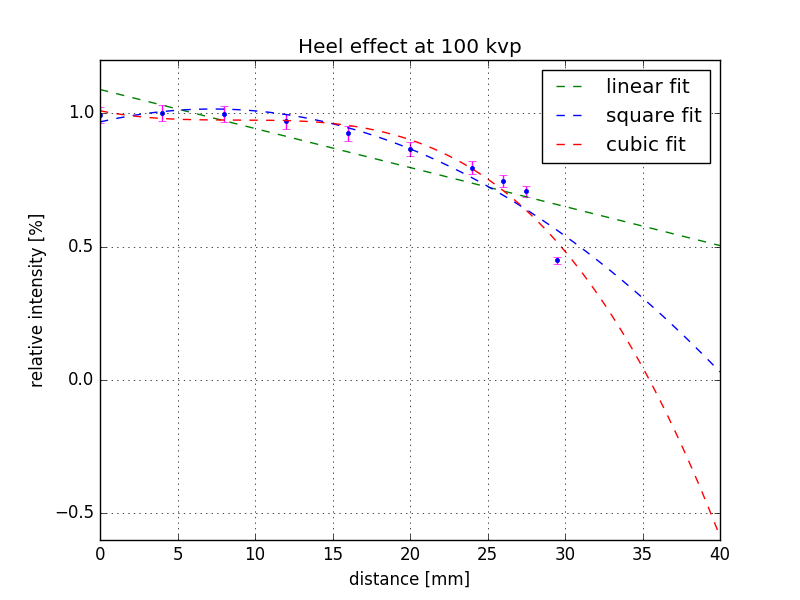
\includegraphics[width=0.75\textwidth]{heel100pvk.png}
\caption{Effetto Heel.}
\end{figure}
	
\section{Referenze}
Il repositorio su GitHub in cui vi sono immagini, programmi Python e Root è https://github.com/Jake145/Gruppo3-Lab-Fisica-Medica.git

\end{document}